La totalidad del rayo incidente es reflejado. Ocurre cuando una onda pasa de un medio con un índice de refracción más alto a un medio con un índice de refracción más bajo, con un ángulo mayor que el \textbf{ángulo crítico}.

\begin{figure}[H]
  \centering
  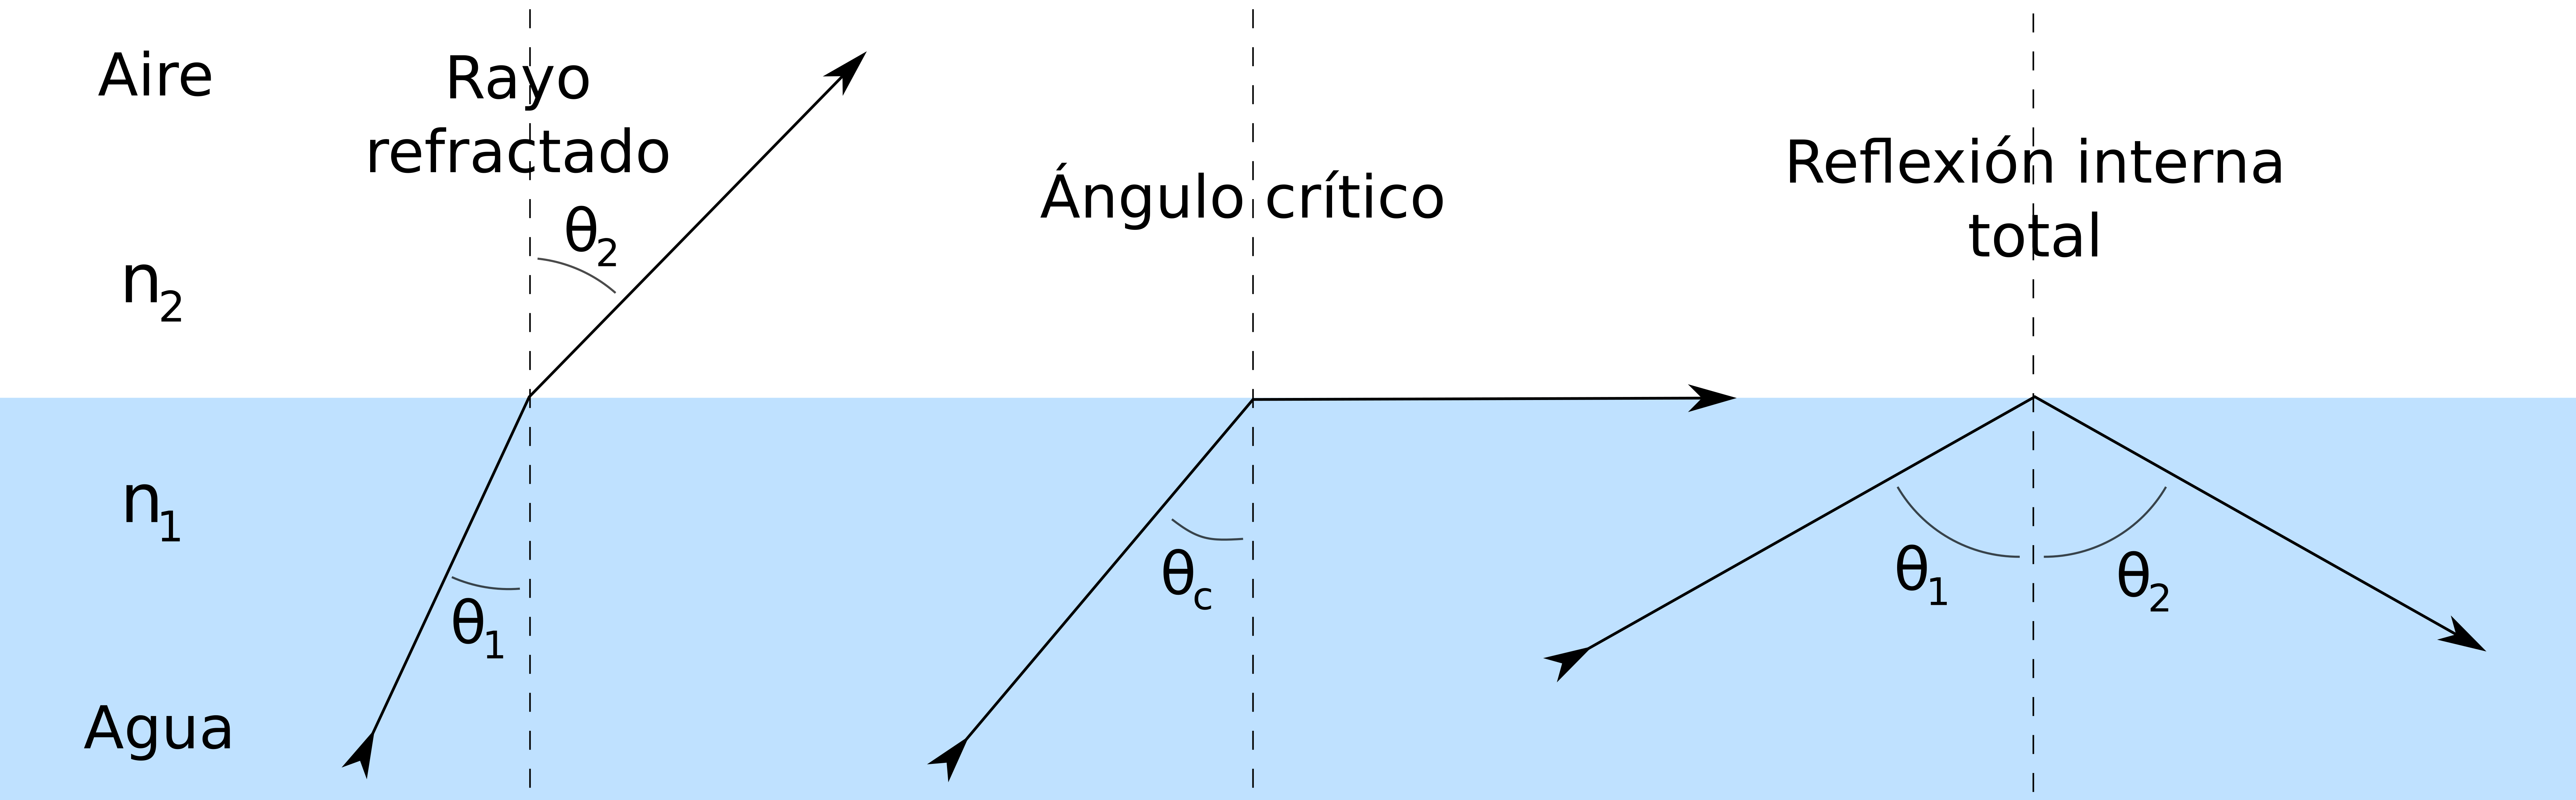
\includegraphics[scale=0.2]{imagenes/reflexion_total_interna.png}
  \caption{Reflexión total interna\cite{wikireftotint}}
\end{figure}

El ángulo crítico $(\theta_c)$ se obtiene de una variación de la ley de Snell, ecuación \ref{equleysnell}, en la cual el ángulo de refracción es de 90 grados $(\sin(90)=1)$. Donde $n_1$ y $n_2$ son los índices de refracción de los medios con $n_2 < n_1$. Se despeja el ángulo de incidencia de la siguiente forma:

\begin{listequbox}
  {\theta_c=\arcsin\left(\dfrac{n_2}{n_1}\right)}{equangcrit}{Ángulo crítico}
\end{listequbox}
